% document formatting
\documentclass[10pt]{article}
\usepackage[utf8]{inputenc}
\usepackage[left=1in,right=1in,top=1in,bottom=1in]{geometry}
\usepackage[T1]{fontenc}
\usepackage{xcolor}

% math symbols, etc.
\usepackage{amsmath, amsfonts, amssymb, amsthm}

% lists
\usepackage{enumerate}

% images
\usepackage{graphicx} % for images

% code blocks
\usepackage{minted, listings} 

% verbatim greek
\usepackage{alphabeta}

\graphicspath{{./assets/images}}

\newcommand{\solution}{\textbf{Solution:}} 
\newcommand{\example}{\textbf{Example: }}

\title{EC ENGR 102 Week 2}

\author{Aidan Jan}
\date{\today}

\begin{document}
\maketitle
\subsection*{The Unit Step Function}
The unit step function denoted by $u(t)$ in this class, is given by:
\[u(t) = \begin{cases} 1 & t \geq 0 \\ 0 & t < 0 \end{cases}\]
It is also called the Heavyside step function.  Drawn below:
\begin{center}
    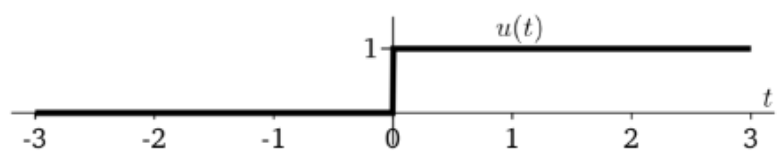
\includegraphics[scale=0.9]{W2_1.png}
\end{center}
\example\\
Suppose I wanted to write
\[x(t) = \begin{cases}e^{-t} & t \geq 1 \\ 0 & t < 1\end{cases}\]
We can do that in terms of the unit step function as
\[x(t) = e^{-t} u(t - 1)\]
\subsubsection*{The Unit Rectangle}
There are two definitions:
\begin{enumerate}
    \item \[rect(t) = \begin{cases} 1 & \vert t \vert < \frac{1}{2} \\ 0 & \text{else} \end{cases}\]
    \begin{itemize}
        \item This is a rectangle with height 1, from t = -0.5 to t = 0.5.
        \item Notice the area under the curve is 1.
    \end{itemize}
    \item \[rect_{\Delta}(t) = \begin{cases} \frac{1}{\Delta} & \vert t \vert < \frac{\Delta}{2}  \\ 0 & \text{else}\end{cases}\]
    \begin{itemize}
        \item This is a general case of the function, where the $\Delta$ represents some number.
        \item $rect_{\Delta}(t)$ where $\Delta = 2$ would make a rectangle going from $t = -1$ to $t = 1$, with height 0.5
        \item Notice that any value of $\Delta$ will still have the area of the rectangle be 1
        \item Most of the time, we use the first definition of rectangle; we use this one for intuition.
    \end{itemize}
\end{enumerate}
\example\\
How do we write the rectangle in terms of $u(t)$?  There are also two ways:
\begin{align*}
    rect(t) &= u(t + 0.5) - u(t - 0.5)\\
    rect(t) &= u(t + 0.5) \cdot u(-t - 0.5)
\end{align*}
We can use the step function and the rectangle function as building blocks for other functions.
\subsection*{Using building blocks}
Consider the following example:
\begin{center}
    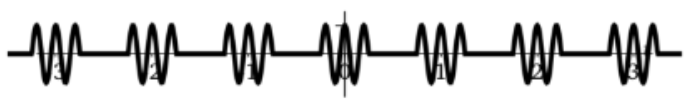
\includegraphics[scale=0.8]{W2_2.png}
\end{center}
How do we write this using the step function as a building block?  Each burst have a form of $A \cos(\omega t)$ and last for a width 0.5 around each integer.\\\\
\textbf{Solution:\\}
The burst around 0 can be written as 
\[rect(2t) \cdot A \cos(\omega t)\]
The burst around 1 can be written as
\[rect(2(t - 1)) \cdot A \cos(\omega t)\]
and et cetera.  As a result, we can write the entire function as:
\[y(t) = \sum_{i = -\infty}^{\infty} rect(2(t - i)) \cdot A\cos(\omega t)\]
\subsection*{Unit Ramp}
The unit ramp is defined as:
\[r(t) = \begin{cases}t & t \geq 0 \\ 0 & t < 0 \end{cases}\]
Note that the unit ramp is the integral of the unit step, i.e.
\[r(t) = \int_{-\infty}^t u(r) \text{d}r\]
The unit ramp is illustrated below:
\begin{center}
    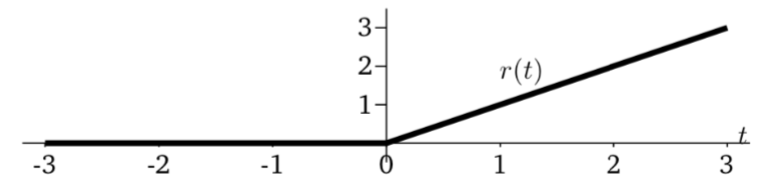
\includegraphics[scale=0.8]{W2_3.png}
\end{center}
This is known in the AI world as ReLU().
\subsubsection*{Unit Triangle}
The unit triangle is defined as:
\[\triangle(t) = \begin{cases}1 - \vert t \vert & \vert t \vert < 1 \\ 0 & \text{else}\end{cases}\]
The unit triangle is illustrated below:
\begin{center}
    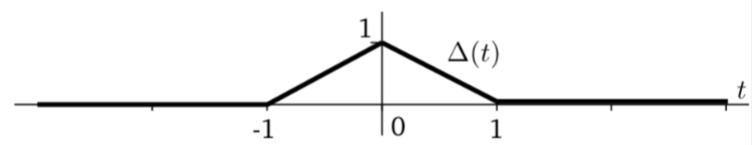
\includegraphics[scale=0.5]{W2_4.png}
\end{center}
\example\\
Lets say we want to make a skewed triangle.  
\begin{center}
    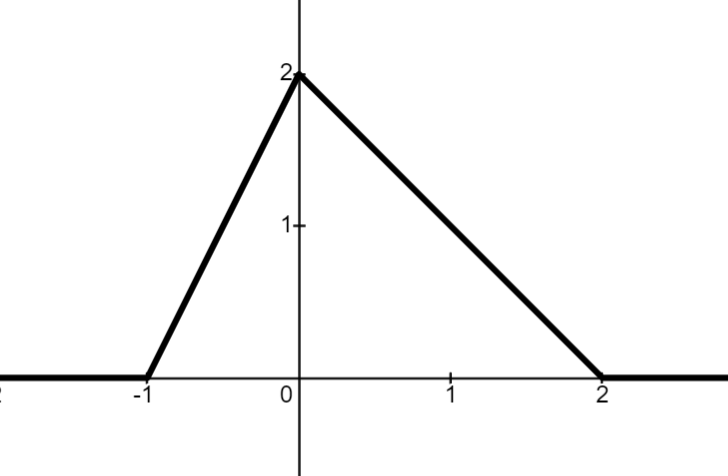
\includegraphics[scale=0.5]{W2_5.png}
\end{center}
\textbf{Solution:\\}
\[x(t) = 2\triangle(t) + \triangle(t - 1)\]
The intuition is the following:
\begin{center}
    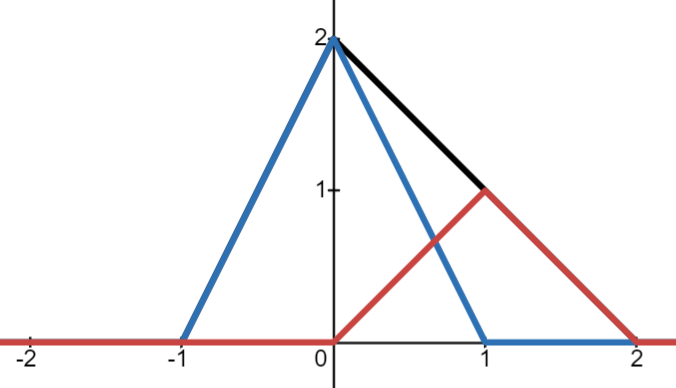
\includegraphics[scale=0.5]{W2_6.png}
\end{center}
The $2\triangle(t)$ term represents the blue line and the $\triangle(t - 1)$ term represents the red line.  We can add the two lines between $0 \geq t \geq 1$ to get the negative 1 slope we need.

\subsection*{Impulse Function}
\textbf{This is an extremely important signal.}
\begin{itemize}
    \item This is defined as $\delta(t)$, or "impulse", "delta", or "Dirac" function.  It is \textbf{not} a rigorous mathematical function.
    \item Features of the impulse function:
    \begin{enumerate} 
        \item It is very large (i.e., approaching infinity), at $t = 0$
        \item It's zero everywhere else, $t \neq 0$.
        \item Area = 1
    \end{enumerate}
    \item Shown on the graph as an arrow pointing up at $t = 0$
\end{itemize}
\begin{center}
    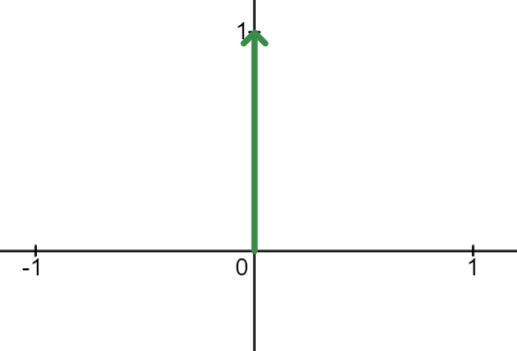
\includegraphics[scale=0.5]{W2_7.png}
\end{center}
\begin{itemize}
    \item The intuition of the impulse function is a $rect_{\Delta}(t)$ where $\Delta$ approaches 0.  (e.g., the width of the rectangle goes to 0 and the height goes to infinity.)
    \item $\delta(t) \cdot x(t) = x(0) \cdot \delta(t)$, where $x(t)$ is any function.
    \begin{itemize}
        \item The impulse is still affected by other functions because by intuition it is a very, very thin rectangle.  The height is an infinitely large number, but not infinity.
        \item The area of the impulse is also scaled by $x(0)$.
        \item The shape of the impulse does not change with scaling, but its area does.
        \item This is called the \textbf{impulse dampening property}.
    \end{itemize}
    \item The impulse can be moved by an amount $T$:
    \[x(t) \cdot \delta(t - T) = x(T) \cdot \delta(t - T)\]
    \begin{itemize}
        \item This is called the \textbf{impulse sampling property}.
    \end{itemize}
    \item What happens when we take the integral?
    \begin{align*}
        &\int_{-\infty}^\infty x(t) \cdot \delta(t) \text{d}t\\
        = &\int_{-\infty}^\infty x(0) \cdot \delta(t) \text{d}t\\
        = &\:x(0) \cdot \int_{-\infty}^\infty \delta(t) \text{d}t\\
        = &\:x(0)
    \end{align*}
    \item What if it is shifted?
    \begin{align*}
        &\int_{-\infty}^\infty x(t) \cdot \delta(t - T) \text{d}t\\
        = &\int_{-\infty}^\infty x(T) \cdot \delta(t - T) \text{d}t\\
        = &\:x(T) \cdot \int_{-\infty}^\infty \delta(t - T) \text{d}t\\
        = &\:x(T)
    \end{align*}
    \[\boxed{\int_{-\infty}^\infty x(t) \delta(t - T) \text{d}t = x(T)}\]
    \begin{itemize}
        \item This is called the \textbf{impulse sifting property}.
    \end{itemize}
\end{itemize}
\subsubsection*{Integral of an impulse}
\begin{align*}
    \int_{\infty}^\infty \delta(t) \text{d}t &= 1\\
    \int_{\infty}^{0+} \delta(t) \text{d}t &= 1\\
    \int_{\infty}^{0-} \delta(t) \text{d}t &= 0
\end{align*}
The $0+$ represents approaching zero from the right (e.g., infinitely close to zero on the positive side), and $0-$ represents approaching zero on the left (e.g., infinitely close to zero on the negative side).
\example\\
Given the signal $x(t)$:
\[x(t) = 1 + \delta(t - 1) - 2\delta(t - 2)\]
What is $y(t) = \int_o^t x(\tau) \text{d}\tau$?
\begin{itemize}
    \item Based on the equation, the graph is always one, with an impulse at $t = 1$, and a negative, double impulse at $t = 2$.
    \item If we take the integral (which is continuous), we get a ramp from $0 < t < 1$, then a step of 1 (since area of impulse = 1), then ramp from $1 < t < 2$, then two steps down (since the negative double impulse has area -2), then a ramp continuing to infinity.
    \item The ramp is present because the constant (+1) creates a line with slope 1 on the integral.
\end{itemize}
Graph of the integral:
\begin{center}
    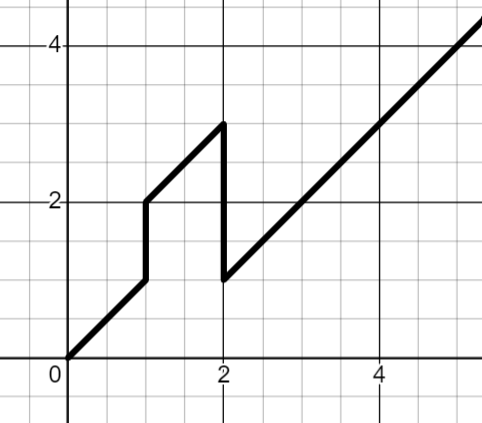
\includegraphics[scale=0.8]{W2_8.png}
\end{center}
\pagebreak
\section*{Systems}
\textbf{What is a system?}\\
A system transforms an \textit{input signal}, $x(t)$, into an output signal, $y(t)$.
\begin{center}
    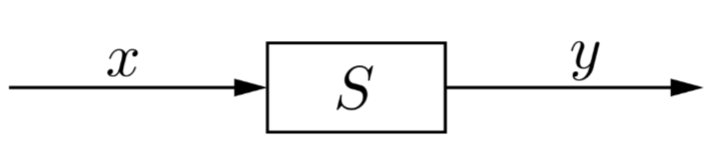
\includegraphics[scale=0.8]{W2_9.png}
\end{center}
\begin{itemize}
    \item Systems, like signals, are also \textit{functions}.  However, their inputs and outputs are signals.
    \item Systems can have either single or multiple inputs (SI or MI, respectively), and single or multiple outputs (SO and MO).  In this class, we focus on \textit{single input, single output} systems (SISO).
\end{itemize}
\subsection*{Example Systems}
\subsubsection*{Scaling System}
Consider an input $x(t)$ and an output $y(t)$.  The scaling system is:
\[y(t) = ax(t)\]
with the following properties:
\begin{itemize}
    \item If $|a| > 1$, the system is called an \textit{amplifier}.
    \item If $|a| < 1$, the system is called an \textit{attenuator}.
    \item If $a < 0$, the system is called \textit{interventing}.
    \item It is common that a block diagram denotes this with a triangle.
\end{itemize}
\begin{center}
    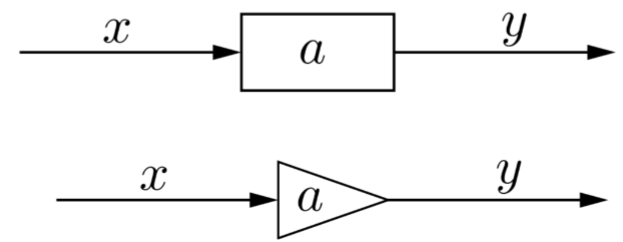
\includegraphics[scale=0.8]{W2_10.png}
\end{center}
\subsubsection*{Differentiator}
The differentiator is denoted:
\begin{align*}
    y(t) &= x'(t)\\
    &= \frac{\text{d}}{\text{d}t} x(t)
\end{align*}
Block diagram below:
\begin{center}
    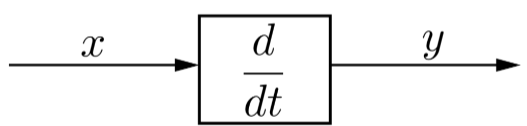
\includegraphics[scale=0.8]{W2_11.png}
\end{center}
\subsubsection*{Integrator}
The integrator is denoted:
\[y(t) = \int_a^t x(\tau) \text{d}\tau\]
where $a$ is often 0 or $-\infty$.\\
Block diagram below:
\begin{center}
    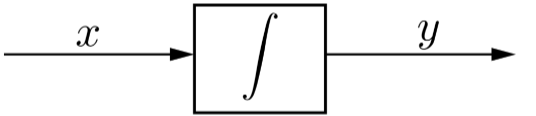
\includegraphics[scale=0.8]{W2_12.png}
\end{center}
\subsubsection*{Time Shift System}
The time shift system shifts a signal by $T$, i.e., 
\[y(t) = x(t - T)\]
\begin{itemize}
    \item If $T > 0$, then it is a \textit{delay} system.
    \item If $T < 0$, then it is a \textit{predictor} system.
\end{itemize}
\subsubsection*{Squarer}
The squarer system squares a signal, i.e.,
\[y(t) = x^2(t)\]
Block diagram below:
\begin{center}
    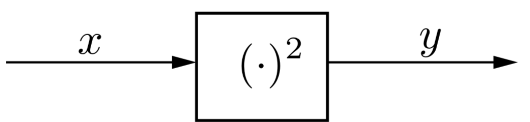
\includegraphics[scale=0.8]{W2_13.png}
\end{center}
\subsubsection*{Systems with multiple inputs}
The AM system (radios) is an example of a system that takes two input signals, $x(t)$ and $\cos(\omega_c t)$, and outputs one signal, $y(t)$.  This is a multiple input, single output (MISO) system.  Here are a few other examples of multiple input systems.
\begin{itemize}
    \item Summing system: $y(t) = x_1(t) + x_2(t)$
    \item Difference system: $y(t) = x_1(t) - x_2(t)$
    \item Multiplier system: $y(t) = x_1(t)x_2(t)$
\end{itemize}
\begin{center}
    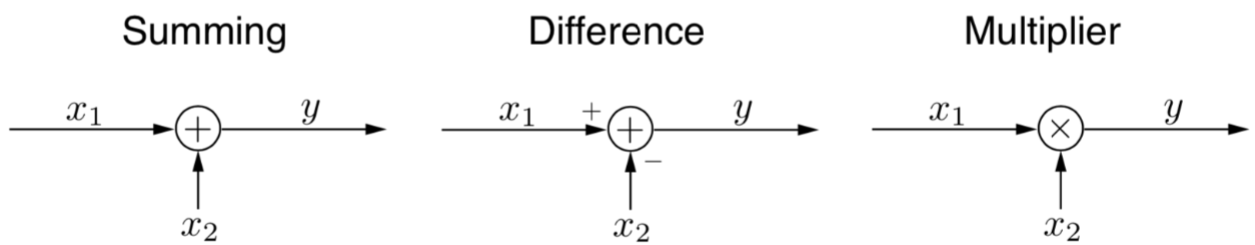
\includegraphics[scale=0.6]{W2_14.png}
\end{center}
\subsubsection*{Amplitude modulation (AM radio)}
Amplitude modulation takes an input "message", $x(t)$ and outputs a "transmitted signal", $y(t)$.  This is denoted via:
\[y(t) = x(t) \cos(2\pi f_c t)\]
Here, $f_c$ is called the carrier frequency.  When you turn to AM radio at e.g., 880 kHz, that means the carrier frequency is $f_c = 880 kHz$.  The AM block diagram is shown below.
\begin{center}
    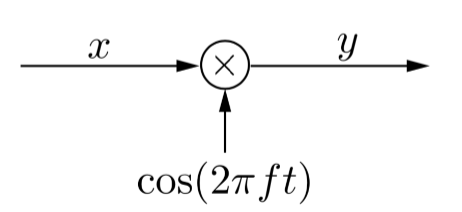
\includegraphics[scale=0.8]{W2_15.png}
\end{center}
\subsection*{System Stability}
A system is \textit{bounded-input, bounded-output} (BIBO) stable if every bounded input leads to a bounded output.
\begin{itemize}
    \item Bounded input: $x(t)$ is a bounded input if there exists a constant $M_x$, such that $|x(t)| < M_x < \infty$ for all $t$.
    \item Boudned output: $y(t)$ is a bounded output if there exists a constant $M_y$, such that $|y(t)| < M_y < \infty$ for all $t$.
    \item Essentially, a system is BIBO stable if both the input and output is always finite and between some threshold value.
    \begin{itemize}
        \item In real life, a non-BIBO stable system can cause electrical fires if the output voltage is too high.
    \end{itemize}
\end{itemize}
\example\\
\underline{AM Radio:} $y(t) = x(t) \cdot \cos(\omega_c t)$
Assume that $|x(t)| < M_x < \infty$.
Then, 
\begin{align*}
    |y(t)| &= |x(t) \cdot \cos(\omega_c t)| \\
    &= |x(t)| \cdot |\cos(\omega_c t)| \\
    &\leq |x(t)| \cdot 1\\
    &\leq M_x
\end{align*}
Therefore, AM radio is BIBO stable.\\
\example\\
\underline{Hyperbola:} $y(t) = \frac{1}{x(t)}$
This function is not BIBO stable - if $x(t) = 0$, $x(t)$ is a bounded input, but $y(t)$ is not a bounded output.
\subsubsection*{What to look for:}
\begin{itemize}
    \item $x(t) < |x(t)|$
    \item Triangle inequality: $\left|\sum_i x_i \right| \leq \sum_i \vert x_i \vert$
    \item $\left| \int_{t_1}^{t_2} x(\tau) \text{d}\tau \right| \leq \int_{t_1}^{t_2} x(\tau) \text{d}\tau$
\end{itemize}

\subsection*{Causal Systems}
\begin{itemize}
    \item A system is causal if its output only depends on past and present values of the input.
    \item All real world systems are causal (i.e., we can't use information from the future).  An example of a non-causal system is the system $x(-t) = S(x(t))$.
\end{itemize}

\subsection*{Time Invariance}
A system is \textit{time invariant} if a time shift in the input only produces an identical time shift of the output.\\
i.e., $S$ is time invariant if
\[y(t) = S(x(t)) \Rightarrow y(t - \alpha) = S(x(t) - \alpha)\]
\example\\
\underline{Squarer:} $y(t) = [x(t)]^2$\\
\begin{itemize}
    \item Let's say we shift the input: $x(t) \rightarrow x(t - \alpha)$
    \item Then, if the function is time invariant, the output becomes $[x(t - \alpha)]^2$.
    \item To check, we shift output.  $y(t) \rightarrow y(t - \alpha) = [x(t - \alpha)]^2$.
    \item They match, therefore, the function is time invariant.
\end{itemize}
\example\\
\underline{AM Radio:} $y(t) = x(t) \cdot \cos(\omega_c t)$
\begin{itemize}
    \item We shift the input: $x(t - \alpha)$
    \item If the function is time invariant, the output becomes $x(t - \alpha) \cdot \cos(\omega_c t)$.
    \item Shift output: $y(t - \alpha) = x(t - \alpha) \cdot \cos(\omega_c (t - \alpha))$
    \item Since they don't match, this function is not time invariant.
\end{itemize}
\subsection*{Linearity}
A system is \textit{linear} if the following two properties hold:
\begin{enumerate}
    \item \textbf{Homogeneity:} for any signal, $x$, and any scalar $a$,
    \[S(ax) = aS(x)\]
    \item \textbf{Superposition:} for any two signals, $x$ and $\widetilde{x}$,
    \[S(x + \widetilde{x}) = S(x) + S(\widetilde{x})\]
    \item To check if a system is linear, we can combine:
    \[S(ax + b\widetilde{x}) = a \cdot S(x) + b \cdot S(\widetilde{x})\]
\end{enumerate}
\example\\
\underline{AM radio:} $y(t) = x(t) \cdot \cos(\omega_c t) = AM(x(t))$.\\
Show that: $AM(ax(t) + b\widetilde{x}(t)) = a \cdot AM(x(t)) + b \cdot AM(\widetilde{x}(t))$.\\
\textbf{Left hand side:}
\begin{align*}
    \text{LHS} &= (ax(t) + b\widetilde{x}(t)) \cdot \cos(\omega_c t) \\
    &= ax(t) \cdot \cos(\omega_c t) + b\widetilde{x}(t) \cdot \cos(\omega_c t) \\
    &= a \cdot AM(x(t)) + b \cdot AM(\widetilde{x}(t))\\
    &= \text{RHS}
\end{align*}
Therefore, AM radio is linear.\\\\
\example\\
\underline{Squarer}: $y(t) = [x(t)]^2$
\begin{align*}
\text{LHS} &= (ax(t) + b\widetilde{x}(t))^2 = a^2x^2(t) + 2abx(t)\widetilde{x}(t) + b^2\widetilde{x}^2(t)\\
\text{RHS} &= a \cdot x^2(t) + b \cdot \widetilde{x}^2(t)
\end{align*}
Since they are not equal, the squarer system is nonlinear.


\end{document}
